%-------------------------------------------------------------------------------
%-------------------------------------------------------------------------------
\chapter{Piles}
%-------------------------------------------------------------------------------
%-------------------------------------------------------------------------------
%-------------------------------------------------------------------------------
\begin{abstract}
    Dans ce chapitre nous allons mettre en évidence dans l'usage de la récursivité une structure de données : les piles. Nous allons ensuite définir et utiliser celle-ci dans d'autres contextes. Une dernière partie définit une autre structure de données : les files.
\end{abstract}
%-------------------------------------------------------------------------------
%-------------------------------------------------------------------------------
%-------------------------------------------------------------------------------
\section{Introduction}
%-------------------------------------------------------------------------------
%-------------------------------------------------------------------------------
\subsection{Récursivité}
%-------------------------------------------------------------------------------
On part de l'algorithme classique du calcul récursif de $a^n$.
\begin{lstlisting}
def puissance(a,n):
    if n <= 0:
        return 1
    else:
        return a*puissance(a,n-1)
\end{lstlisting}

On a les évaluations suivantes
\begin{lstlisting}
>>> puissance(1.007, 900)
532.7500489085279
>>> puissance(1.007, 1000)
Traceback (most recent call last):
  File "<console>", line 1, in <module>
  File "<tmp 1>", line 5, in puissance
    return a*puissance(a,n-1)
  File "<tmp 1>", line 5, in puissance
    return a*puissance(a,n-1)
  File "<tmp 1>", line 5, in puissance
    return a*puissance(a,n-1)
  [Previous line repeated 984 more times]
  File "<tmp 1>", line 2, in puissance
    if n <= 0:
RecursionError: maximum recursion depth exceeded in comparison
\end{lstlisting}

Le message d'erreur est impressionnant par sa longueur.

Il nous parle d'une profondeur maximale de récursivité dépassée.

De quoi s'agit-il ?

Lors de l'appel de \type{puissance(1.007, 1000)} la fonction doit calculer \type{puissance(1.007, 999)}. Pendant qu'elle calcule cette valeur
elle doit se souvenir qu'elle doit multiplier le résultat par $1.007$, elle met donc cette opération "en attente".

Lorsqu'elle calcule \type{puissance(1.007, 999)} elle doit aussi considérer le nouveau produit par $1.007$ comme inachevé, il faut le mémoriser.

En poursuivant ainsi on voit qu'on doit mettre 1000 fois en attente la multiplication par $1.007$.

Dans chaque langage il y a une limite au nombre de calculs que l'on peut mettre en attente. Pour python cette limite est inférieure à 1000.

\medskip

On détaille cette mise en suspend des calculs avec un autre algorithme récursif.
\begin{lstlisting}
def fact(n):
    if n <= 0:
        return 1
    else:
        return n*fact(n-1)
\end{lstlisting}

Lors du calcul de \type{fact(3)} le programme doit calculer \type{fact(2)} en conservant la multiplication par 3 en mémoire, il écrit donc cette opération en réserve.

De même le calcul de \type{fact(2)} met le produit par 2 en attente, puis le calcul de \type{fact(1)} suspend le produit par 1  et on arrive à \type{fact(0)} qui donne immédiatement 1. On peut alors calculer pas-à-pas le résultat en lisant les calculs mis en attente ; on commence par le dernier calcul mémorisé et on finit lors qu'il n'y a plus rien.
%--------------------------------------------------------------------------
\begin{center}
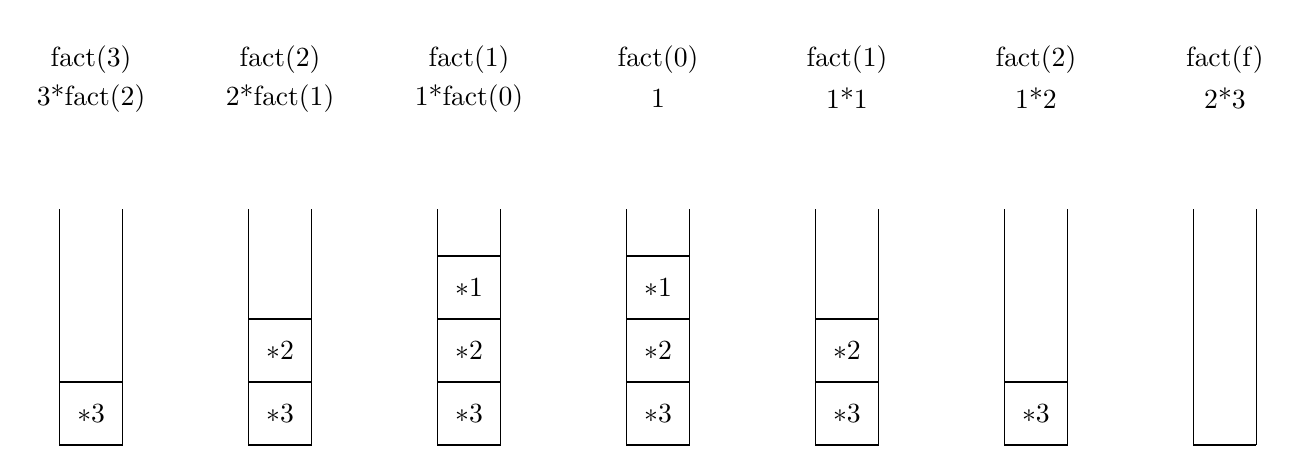
\begin{tikzpicture}
\tikzstyle{every node}=[minimum size =8mm]
\foreach \i/\txt/\f in {0/3*fact(2)/3,  1/2*fact(1)/2, 2/1*fact(0)/1, 3/1/0, 4/1*1/1, 5/1*2/2, 6/2*3/f}
  {\node (f\i)  at ({2.4*\i},4.5) {\type{fact(\f)}};
   \node (g\i)  at ({2.4*\i},4) {\type{\txt}};
   \draw ({\i*2.4-0.4},-0.4) -- +(0,3);
   \draw ({\i*2.4+0.4},-0.4) -- +(0,3);};
\foreach \i in {0,1,...,5}  \node[draw] (x3) at ({\i*2.4},0) {$*3$};
\foreach \i in {1,2,...,4}  \node[draw] (x2) at ({\i*2.4},0.8) {$*2$};
\foreach \i in {2,3}  \node[draw] (x1) at ({\i*2.4},1.6) {$*1$};
\draw (14,-0.4) -- +(0.8, 0);
\end{tikzpicture}
\end{center}
%--------------------------------------------------------------------------
%-------------------------------------------------------------------------------
\subsection{Une structure de données}
%-------------------------------------------------------------------------------
  \begin{center}
    \includegraphics{5_pileDossiers}
  \end{center}

On voit donc que la récursivité utilise une structure de données qui peut accumuler les données et qui en restitue une à la fois en commençant par la dernière donnée ajoutée. L'acronyme anglais, {\bf LIFO} pour Last In, First Out, exprime bien cette idée que le premier sorti est le dernier entré. 
On parlera de {\bf pile} pour ce type de données, ce qui correspond à l'idée d'empiler les données en attente.

\medskip

Une pile est utilisée dans d'autres contextes.

\begin{itemize}
\item Dans un navigateur web, une pile sert à mémoriser les pages Web visitées. L'adresse de chaque nouvelle page visitée est empilée et l'utilisateur dépile l'adresse de la page précédente en cliquant le bouton ``Afficher la page précédente.''
\item L'évaluation des expressions mathématiques en notation post-fixée (ou polonaise inverse) utilise une pile, voir la partie \ref{app:parentheses}.
\item La vérification du bon parenthésage d'une expression se fait en complexité linéaire avec une pile, voir la partie \ref{app:npi}.
\item La fonction ``Annuler la frappe'' (Undo) d'un traitement de texte mémorise les modifications apportées au texte dans une pile.
\end{itemize}

\medskip

Nous allons donner plusieurs moyens de définir en Python une structure de donnée qui correspond à la pile. Mais, avant de le faire, nous allons définir de manière abstraite ce que l'on veut. Cette méthode permettra de pouvoir passer d'une implémentation à une autre sans se préoccuper des détails internes : toutes les implémentations devront être conformes au cadre imposé. En contrepartie on s'interdira d'utiliser les subtilité de telle ou telle écriture. 
%-------------------------------------------------------------------------------
%-------------------------------------------------------------------------------
\section{Type de données abstrait}
%-------------------------------------------------------------------------------
%-------------------------------------------------------------------------------
\subsection{Définitions}
%-------------------------------------------------------------------------------
Le langage python fournit des structures de données comme les listes, tuples et chaînes de caractères, le module \type{numpy} fournit un type de tableaux. Chaque type de données a ses  avantages et ses contraintes propres. Il est judicieux de chercher d'abord la structure de données adaptée à la problématique : choisir  une chaîne de caractère, une liste ou un tableau \type{numpy} peut changer beaucoup d'aspects du programme, comme les complexités spatiale et temporelle du programme.

Nous allons ici renverser la perspective : au lieu d'utiliser des données avec leur caractéristiques imposées par le langage, nous allons définir les propriétés souhaitées et les implémenter dans le langage considéré. Ces propriétés forment le {\bf type de données abstrait}, les implémentations seront un type de données concret.


La spécification d'un type de donnée abstrait est composée  :
\begin{itemize}
\item de la définition d'un certain nombre d'opérations concernant le type de données,
\item des axiomes qui définissent le comportement,
\item des préconditions si les opérations sont partiellement définies.
\end{itemize}

Les fonctions de manipulation des structures de données sont de trois classes : 

\begin{itemize}
\item les {\it constructeurs} qui permettent de créer des ensembles et d'ajouter des éléments,
\item les {\it prédicats} qui sont des fonctions dont le résultat est \type{True} ou \type{False},
\item les fonctions de  {\it sélection} qui permettent d'extraire certains éléments et informations. 
\end{itemize}

Il existera un choix important à faire lorsque l'on utilisera une structure de données dans laquelle on peut ajouter des éléments. 

\begin{itemize}
\item Soit on ajoute un élément à un ensemble en conservant l'ensemble, c'est ce que l'on fait par exemple avec la méthode \type{append} qui modifie une liste sans en créer une nouvelle : on parle de données {\bf mutables}. Dans ce cas la structure est un contenant, ce qui est à l'intérieur peut changer.

\item Soit on crée un nouvel ensemble par l’ajout d'un élément : on parle alors de données {\bf persistantes}. 

Dans ce cas la structure est pensée comme l'ensemble des ces éléments, lui ajouter (ou enlever) un élément crée une autre structure.

Les structures persistantes sont peu utilisées en Python (sauf pour les chaînes de caractères).
\end{itemize}
%-------------------------------------------------------------------------------
\subsection{Les piles}
%-------------------------------------------------------------------------------
Nous allons définir un type mutable pour les piles : pour reprendre l'analogie des piles de dossier, un pile est plutôt un ensemble de dossier qui change de jour en jour plutôt qu'une installation en art moderne qui représenterait un bureau sans qu'on puisse jamais y modifier quoi que ce soit.

\medskip

Les spécifications sont assez naturelles.
\begin{itemize}
\item Les constructeurs : 
\begin{itemize}
\item \type{create()} qui renvoie une pile ne contenant aucun élément,
\item \type{push(x, p)} qui ajoute l'élément \type{x} à la pile \type{p} ; cette fonction ne renvoie rien.
\end{itemize}
\item Un prédicat :\type{is\_empty(p)} qui renvoie \type{True} ou \type{False} selon que la pile \type{p} contient des élément ou non.

\item Les fonctions servent à voir le dernier élément ajouté. Il y a deux cas selon que l'on enlève ou non cet élément.
\begin{itemize}
\item \type{pop(p)} retire le dernier ajouté à la pile et le renvoie.
\item \type{top(p)} envoie le dernier élément ajouté à la pile {\bf sans modifier la pile}.
\end{itemize}
\item Ces fonctions ont une précondition : elles ne sont définies que si la pile passée en paramètre est non vide.
\item Les axiomes reflètent les propriétés souhaitées.
\begin{itemize}
\item \type{empty(create())} renvoie \type{True}
\item \type{empty(p)} après \type{push(x, p)} renvoie \type{False}
\item \type{pop(p)} après \type{push(x, p)} renvoie \type{x} et la suite de ces deux instructions fait retourner \type{p} à son état initial.
\end{itemize}
\end{itemize}
On admet que ces axiomes déterminent de manière unique le comportement des fonctions.
%-------------------------------------------------------------------------------
%-------------------------------------------------------------------------------
\section{Piles concrètes}
%-------------------------------------------------------------------------------
%-------------------------------------------------------------------------------
\subsection{Utilisation de listes}
%-------------------------------------------------------------------------------
Les listes Python donnent, de manière naturelle, une structure de pile.
%----------------------------------------------------------------
\begin{lstlisting}
def create():
    return []
    
def push(x, pile):
    pile.append(x)
    
def is_empty(pile):
    preturn pile == []
    
def pop(pile):
    return pile.pop()
    
def top(pile):
    return pile[-1]
\end{lstlisting}
%-------------------------------------------------------------------------------
\newpage
%-------------------------------------------------------------------------------
\subsection{Utilisation de tableaux {\tt numpy}}
%-------------------------------------------------------------------------------
Une pile peut aussi être implémentée dans un tableau de taille fixée comme le sont les tableaux \type{numpy}.

On supposera que le module \type{numpy} a été importé
%-------------------------------------------------------------------------------
\begin{lstlisting}
import numpy as np
\end{lstlisting}
%-------------------------------------------------------------------------------

On remplit les positions libres à partir de 0 ; il faut conserver la position de la dernière case occupée ou de la première case libre. La taille maximale sera fixée à l'avance : on prend le risque d'un dépassement de capacité comme il se produit avec la pile de récursivité.

On choisit ici de considérer la pile comme un couple dont la première composante est le nombre d'éléments dans la pile, c'est l'indice de la première position libre, et la seconde composante est le tableau.

%----------------------------------------------------------------
\begin{lstlisting}[caption = {Fonctions de piles avec un tableau}]
def create():
    nMax = 1000
    tableau = np.zeros(nMax)
    return [0, tableau]
    
def is_empty(pile):
    return pile[0] == 0
    
def push(x, pile):
    n, tableau = pile
    nMax = len(tableau)
    if n < nMax:
        tableau[n] = x
        pile[0] = n + 1
    else:
        print("La pile est pleine")
    
def pop(p):
    n, tableau = pile
    if n > 0:
        x = tableau[n-1]
        pile[0] = n - 1
        return x
    else:
        print("La pile est vide")
        
def pop(p):
    n, tableau = pile
    if n > 0:
        return tableau[n-1]
    else:
        print("La pile est vide")
\end{lstlisting}
%-------------------------------------------------------------------------------
\newpage
%--------------------------------------------------------------------------
\subsection{Utilisation d'objets}
%--------------------------------------------------------------------------
Nous allons ici ébaucher l'utilisation de la programmation objet.

\medskip

On peut voir une pile comme une chaîne de valeurs dont on ne connaît que la dernière

%--------------------------------------------------------------------------
\begin{center}
\begin{tikzpicture}[scale = 0.8,grand/.style={minimum height=0.8cm, minimum width=1.6cm}]
\foreach \i/\v in {0/4, 1/7, 2/11, 3/-4, 4/2}
  \node[grand,draw] (t\i) at (3*\i, 0) {\v};
\foreach \i in {1,2,3,4}
  {\pgfmathsetmacro\j{int(\i - 1)}
  \draw (t\i) -- (t\j);};
\draw [<-] (t4.north) -- +(0,0.8) node[above= -1mm]{\tt dernier};
\end{tikzpicture}
\end{center}
%-------------------------------------------------------------------------------
Quand on ajoute un élément, il devient le dernier. 

Pour retirer un élément il faut retrouver le précédent ; chaque élément devra donc être associé à son précédent

%--------------------------------------------------------------------------
\begin{center}
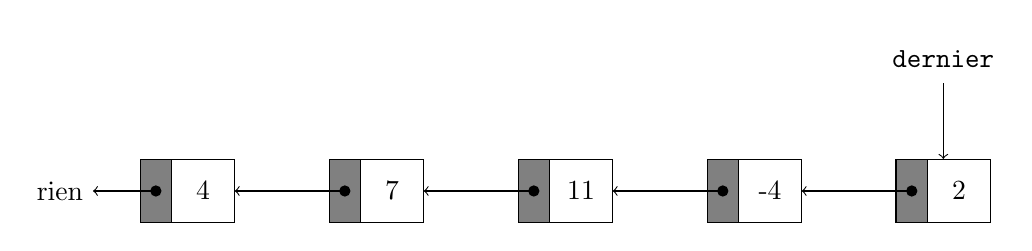
\begin{tikzpicture}[scale = 0.8,
                  grand/.style={minimum height=0.8cm, minimum width=1.2cm},
                  petit/.style={minimum size=0.8cm}]
\foreach \i/\v in {0/4, 1/7, 2/11, 3/-4, 4/2}
  {\node[grand,draw,fill=gray] (t\i) at (3*\i-0.25, 0) {};
   \node[petit,draw,fill=white] (tt\i) at (3*\i, 0) {\v};};
\foreach \i in {0,1,...,4}
  \draw[fill] (\i*3-0.75,0) circle (0.08);
\foreach \i in {1,2,3,4}
   \draw[->] (\i*3-0.75,0) -- ++(-1.75,0);
\draw[->] (-0.75,0) -- ++(-1,0) node[left] {rien};
\draw [<-] (t4.north) -- +(0,1.2) node[above= -1mm]{\tt dernier};
\end{tikzpicture}
\end{center}
%-------------------------------------------------------------------------------
Dans les langages à objet comme Python on peut définir naturellement une structure de pile. 

C'est une {\bf classe} doit contenir une valeur et la pile "en dessous".

On peut remarquer que la définition est récursive.

Lorsque l'élément est le premier on indique \type{None} pour signifier qu'il n'y a rien en dessous : \type{None} est donc l'élément terminal.

La classe est définie par méthode de création, appelée \type{\_\_init\_\_}
%-------------------------------------------------------------------------------
\begin{lstlisting}
class Pile:
    def __init__(self, x):
        self.valeur = x
        self.avant = None
\end{lstlisting}
%-------------------------------------------------------------------------------
Le nom \type{self} pour la variable est usuel.

On créera un élément par \type{e = Pile(5)}, par exemple. 

Lors de sa création l'élément n'a pas de prédécesseur.

La pile de l'exemple ci-dessus peut être définie par \type{e5}
%-------------------------------------------------------------------------------
\begin{lstlisting}
e1 = Element(4)
e2 = Element(7)
e2.avant = e1
e3 = Element(11)
e3.avant = e2
e4 = Element(-4)
e4.avant = e3
e5 = Element(2)
e5.avant = e4
\end{lstlisting}
%-------------------------------------------------------------------------------
C'est en fait une pile persistante, quand on ajoute un élément on crée une nouvelle pile.

Pour définir une pile mutable il suffit de définir un contenant de pile.

Ce sera aussi une classe, c'est un objet qui réfère au dernier élément.
\begin{lstlisting}
class Stack:
    def __init__(self):
        self.dernier = None
\end{lstlisting}

Ici une pile créée sera supposée vide.

\newpage
Pour ajouter une valeur $x$ à une pile 
\begin{itemize}
\item on crée l'élément associé à x
\item son prédécesseur est l'élément associé à la pile
\item la pile est maintenant associée à ce nouvel élément.
\end{itemize}
%----------------------------------------------------------------
\begin{lstlisting}[caption = {Fonctions de piles avec des objets}]
def create():
    return Stack()
    
def is_empty(pile):
    return pile.dernier is None

def push(x, pile):
    e = Pile(x)
    penult = pile.dernier
    e.avant = penult
    pile.dernier = e
   
def pop(pile):
    if is_empty(pile):
        print("La pile est vide")
    else:
        bout = pile.dernier
        pile.dernier = bout.avant
        return bout.valeur
   
def top(pile):
    if is_empty(pile):
        print("La pile est vide")
    else:
        return pile.dernier.valeur
\end{lstlisting}
%-------------------------------------------------------------------------------
\newpage
%--------------------------------------------------------------------------
\section{Applications}
%-------------------------------------------------------------------------------
%-------------------------------------------------------------------------------
Dans cette partie on donne, sous forme d'exercices, quelques applications des piles.
%-------------------------------------------------------------------------------
%-------------------------------------------------------------------------------
\subsection{Parenthésages}\label{app:parentheses}
%-------------------------------------------------------------------------------
On veut étudier le parenthésage d'expressions arithmétiques ou du code source d'un programme. Il est utile de vérifier que les parenthèses sont bien écrites et aussi de déterminer la parenthèse ouvrante associée à une parenthèse fermante.

Par exemple $1 + 2*(7-(4-3)*((2-5)+2*((12/4-8)+2*3)))$ est bien parenthésée et la parenthèse ouvrante après $(4-3)*$ est associée à l'avant dernière parenthèse fermante.

On considère une chaîne de caractère représentant l'expression et on s'intéresse uniquement aux parenthèses classiques "(" et ")".

Pour savoir si une expression est bien parenthésée il faut vérifier qu'il y a autant de parenthèses ouvrantes que de parenthèses fermantes et que chaque parenthèse fermante est associée à une parenthèse ouvrante placée avant elle. Celle-ci est la dernière parenthèse ouvrante du texte non encore fermée. On voit apparaître l'utilité d'une pile.

\begin{itemize}
\item On lit les caractères un par un,
\item quand on voit une parenthèse ouvrante on empile sa position
\item quand on lit une parenthèse fermante on dépile un élément, il sera la position de la parenthèse ouvrante associée.
\item Si on doit dépiler alors que la pile est vide ou si la pile est non vide à la fin c'est que l'expression n'est pas bien parenthésée.
\end{itemize}

Dans la chaîne "1+2*(7-(4-3)*((2-5)+2*((12/4-8)+2*3)))" correspondant à l'expression ci-dessus les opérations de la pile seront 
\begin{itemize}
\item on empile 4,
\item on empile 7 
\item on dépile 7 qui est associé à 11
\item on empile 13 
\item on empile 14 
\item on dépile 14 qui est associé à 18
\item on empile 22 
\item on empile 23
\item on dépile 23 qui est associé à 30
\item on dépile 22 qui est associé à 35
\item on dépile 13 qui est associé à 36
\item on dépile 4 qui est associé à 37.
\end{itemize}

On peut donner le résultat sous la forme d'une liste de couples, pour l'exemple ci-dessus on aurait, comme résultat, la liste 

\type{[(7, 11), (14, 18), (23, 30), (22, 35), (13, 36), (4, 37)]}.
%-------------------------------------------------------------------------------
%-------------------------------------------------------------------------------
\begin{Exercise}[title = {Liste des parenthèses associées}]\it

Écrire une fonction \type{listePar} qui reçoit une expression {\bf supposée bien parenthésée} et qui retourne la liste des couples d'indices de parenthèses associées.
\end{Exercise} 
%-------------------------------------------------------------------------------
\begin{Answer}
\begin{lstlisting}
def listePar(ch):
    n = len(ch)
    l = []
    p = create()
    for i in range(n):
        if ch[i] == "(":
            push(i, p)
        if ch[i] == ")":
            j = pop(p)
            l.append((j,i))
    return l
\end{lstlisting}
\end{Answer}
%-------------------------------------------------------------------------------
%-------------------------------------------------------------------------------
\begin{Exercise}[title = {Test de parenthésage}]\it

Écrire une fonction \type{bienPar} qui reçoit une expression qui n'est plus supposée bien parenthésée et qui renvoie \type{True} ou \type{False} selon que la liste est bien parenthésée ou non.
\end{Exercise} 
%-------------------------------------------------------------------------------
\begin{Answer}
Il suffit de compter les parenthèses ouvrantes non encore fermées ; on n'a pas besoin d'une pile.
\begin{lstlisting}
def bienPar(ch):
    n = len(ch)
    ouvrantes = 0
    for i in range(n):
        if ch[i] == "(":
            ouvrantes = ouvrantes + 1
        if ch[i] == ")":
            if ouvrantes == 0:
                return False
            else:
                ouvrantes = ouvrantes - 1
    return ouvrantes == 0
\end{lstlisting}
\end{Answer}
%-------------------------------------------------------------------------------
%-------------------------------------------------------------------------------
\begin{Exercise}[title = {Liste des parenthèses associées et parenthèse isolée}]\it

Modifier la fonction \type{listePar} pour qu'elle renvoie une liste de couples contenant tous les indices de parenthèses même si le texte n'est pas bien parenthésé.

Une parenthèse fermante qui n'est pas associée à une parenthèse ouvrante sera renvoyée sous la forme sous la forme \type{(-1 ,i)} et une parenthèse ouvrante non associée à une parenthèse fermante sera renvoyée sous la forme \type{(i, -1)}.
\end{Exercise} 
%-------------------------------------------------------------------------------
\begin{Answer}
\begin{lstlisting}
def listePar(ch):
    n = len(ch)
    l = []
    p = create()
    for i in range(n):
        if ch[i] == "(":
            push(i, p)
        if ch[i] == ")":
            if empty(p):
                l.append((-1,i))
            else:
                j = pop(p)
                l.append((j,i))
    while not(empty(p)):
        j = pop(p)
        l.append((j,-1))
    return l
\end{lstlisting}
\end{Answer}
%-------------------------------------------------------------------------------
%-------------------------------------------------------------------------------
Par exemple \type{listePar("(1+2))*((5-3)")} renverra \type{[(0, 4), (-1, 5), (9, 12), (8, -1)]},
%-------------------------------------------------------------------------------
%-------------------------------------------------------------------------------
\subsection{Notation post-fixée (ou polonaise inversée)}\label{app:npi}
%-------------------------------------------------------------------------------
En 1920 le mathématicien polonais Jan Lukasiewicz propose la notation pré-fixé (ou polonaise) qui consiste à considérer les opérations comme des opérateurs à 2 variables, $7 + 11$ s'écrit $+\; 7\; 11$. L'avantage est que les parenthèses deviennent inutiles :

 $(7-2).\sin(2x+\pi/3)$ devient
$*\; -\; 7\; 2\; \sin\; +\; *\; 2\; x\; /\; \pi\; 3$.

La notation polonaise inverse ou notation post-fixée a été proposée par le philosophe et informaticien australien Charles Leonard Hamblin  dans le milieu des années 1950. 

Elle a été diffusée dans le public comme interface utilisateur avec les calculatrices de bureau de Hewlett-Packard (HP-9100), puis avec la calculatrice scientifique HP-35 en 1972.

Elle consiste simplement à placer l'opérateur {\bf après} les deux opérande, $7 + 11$ s'écrit $7\; 11\; +$. L'expression $32 - 2 (12 - 3 (7 - 2))$ peut s'écrire
$32\;  2\;  12\;  3\;  7\;  2\;  -\;   *\;  -\;  *\;  -$

L'avantage est que, combinée à une pile, cette notation permet d'effectuer les calculs sans faire référence à une quelconque adresse mémoire. 

\begin{itemize}
\item On lit l'expression terme-à-terme :

\item si on lit une valeur numérique, elle est empilée, 

\item si on lit une opération $\clubsuit$, 

on dépile les deux derniers opérandes $a$ et $b$ 

et on empile le résultat du calcul $a \clubsuit b$.
\end{itemize}	
%-------------------------------------------------------------------------------
%-------------------------------------------------------------------------------
\begin{Exercise}[title = {Un exemple}]\it

Simuler l'évolution de la pile avec l'expression $32\;  2\;  12\;  3\;  7\;  2\;  -\;  *\;  -\;  *\;  -$
\end{Exercise} 
%-------------------------------------------------------------------------------
\begin{Answer}
Après avoir empilé les nombres on lit les opérateurs.
\begin{itemize}
\item La pile contient 32, 2, 12, 3, 7, 2.
\item On dépile 2 puis 7, on calcule $7-2=5$ (attention à l'ordre), on empile 5.
\item La pile contient 32, 2, 12, 3, 5.
\item On dépile 5 puis 3, on calcule $3.5=15$, on empile 15.
\item La pile contient 32, 2, 12, 15.
\item On dépile 15 puis 12, on calcule $12-15=-3$, on empile $-3$.
\item La pile contient 32, 2, $-3$.
\item On dépile $-3$ puis 2, on calcule $2.(-3)=-6$, on empile $-6$.
\item La pile contient 32, $-6$.
\item On dépile $-6$ puis 32, on calcule $32-(-3)=38$, on empile $38$.
\item La pile contient 38 qui est le résultat renvoyé.
\end{itemize}
\end{Answer}%-------------------------------------------------------------------------------
%-------------------------------------------------------------------------------
\begin{Exercise}[title = {Simulation d'une calculatrice}]\it

Écrire une fonction \type{npi(liste)} qui prend en entrée une liste contenant des valeurs numériques et des chaînes \type{'+', '-', '*', '/'} et qui calcule la valeur de l'expression en NPI. On considère que les nombres sont des flottants, la division est la division réelle classique.

Pourquoi est-il difficile de lire directement une chaîne de caractères pour l'évaluer ?
\end{Exercise} 
%-------------------------------------------------------------------------------
\begin{Answer}
\begin{lstlisting}
def npi(liste):
    p=creerPile()
    for x in liste:
        if x == '+' :
            b = pop(p)
            a = pop(p)
            push(a + b, p)
        elif x == '-' :
            b = pop(p)
            a = pop(p)
            push(a + b, p)
        elif x == '*' :
            b = pop(p)
            a = pop(p)
            push(a * b, p)
        elif x == '/' :
            b = pop(p)
            a = pop(p)
            push(a . b, p)
        else:
            push(x, p)
    return pop(p)
\end{lstlisting}

Le problème de la lecture directe d'une chaîne de caractères est le double sens du signe moins : il est à la fois une opération binaire et un changement de signe.
\end{Answer}
%-------------------------------------------------------------------------------
%-------------------------------------------------------------------------------
\subsection{Files d'attente}
%-------------------------------------------------------------------------------
Une {\it file} ({\it queue} en anglais ) est une structure de données basée sur le principe : premier entré, premier sorti, en anglais {\bf FIFO} (First In, First Out), ce qui veut dire que les premiers éléments ajoutés à la file seront les premiers à en être extraits. 

\begin{center}
\begin{tikzpicture}
 \node[state] (s11) at (0,0) {$8$};
 \node[state] (s12) at (-1,0) {$5$};
 \node[state] (s13) at (-5,0) {$7$};
 \draw (-3.5,0.5)-- ++(4,0);
 \draw (-3.5,-0.5)-- ++(4,0);
 \draw [->](s13.east) -- ++(2,0);
%
 \node[state] (s11) at (0,-1.5) {$8$};
 \node[state] (s12) at (-1,-1.5) {$5$};
 \node[state] (s13) at (-2,-1.5) {$7$};
 \draw (-3.5,-1)-- ++(4,0);
 \draw (-3.5,-2)-- ++(4,0);
 \draw [->](s11.east) -- ++(1,0);
%
 \node[state] (s11) at (0,-3) {$5$};
 \node[state] (s12) at (-1,-3) {$7$};
 \draw (-3.5,-2.5)-- ++(4,0);
 \draw (-3.5,-3.5)-- ++(4,0);
 \draw [->](s11.east) -- ++(1,0);
%
 \node[state] (s11) at (0,-4.5) {$7$};
 \draw (-3.5,-4)-- ++(4,0);
 \draw (-3.5,-5)-- ++(4,0);
%
\end{tikzpicture}
\end{center}{\bf Exemples}
\begin{itemize}
\item Toutes les situations où l'on est servi en fonction de l'ordre d'arrivée sont des files d'attente : passage à la cantine, à un guichet d'administration, au cinéma \dots

\item Les serveurs d'impression, qui doivent traiter les requêtes dans l'ordre dans lequel elles
arrivent, les insèrent dans une file d'attente.

\item Plus généralement on utilise des files pour créer toutes sortes de mémoires tampons (en anglais
buffers).
\end{itemize}

On voit que l'on ajoute les éléments comme dans une pile et qu'on les retire comme dans une pile inversée. On pourrait utiliser une pile en la retournant à chaque fois qu'on a besoin de retirer un élément puis en la reconstituant mais le nombre d'opérations serait trop important. 

Il existe une méthode astucieuse qui utilise 2 piles :
%-------------------------------------------------------------------------------
\begin{itemize}
  \item on ajoute dans la première,
  \item on retire depuis la seconde,
  \item quand la seconde est vide on retourne la première dans la seconde.
\end{itemize}
%-------------------------------------------------------------------------------
Le retournement peut sembler coûteux mais est amorti : chaque élément ne sera retourné qu'une fois.
%-------------------------------------------------------------------------------
\begin{center}
\begin{tikzpicture}
 \node[state] (s11) at (0,0) {$8$};
 \node[state] (s12) at (0,1) {$5$};
 \node[state] (s10) at (1,0) {$7$};
 \node[state] (s13) at (-1,4) {$3$};
 \draw (-0.5,3)-- ++(0,-3.5) -- ++(1,0) -- ++(0,3.5);
 \draw (0.5,3)-- ++(0,-3.5) -- ++(1,0) -- ++(0,3.5);
 \draw [->](s10.north) |- ++(1,3);
 \draw [->](s13.east) -| ++(0.5,-1);
%
 \node[state] (s21) at (3,0) {$8$};
 \node[state] (s22) at (3,1) {$5$};
 \node[state] (s23) at (3,2) {$3$};
 \draw (2.5,3)-- ++(0,-3.5) -- ++(1,0) -- ++(0,3.5);
 \draw (3.5,3)-- ++(0,-3.5) -- ++(1,0) -- ++(0,3.5);
 \draw [->](s23.north) |- ++(1,1) -- ++(0,-2);
%
 \node[state] (s34) at (5,4) {$4$};
 \node[state] (s31) at (7,0) {$3$};
 \node[state] (s32) at (7,1) {$5$};
 \node[state] (s33) at (7,2) {$8$};
 \draw (5.5,3)-- ++(0,-3.5) -- ++(1,0) -- ++(0,3.5);
 \draw (6.5,3)-- ++(0,-3.5) -- ++(1,0) -- ++(0,3.5);
 \draw [->](s34.east) -| ++(0.5,-1);
 \draw [->](s33.north) |- ++(1,1);
\end{tikzpicture}
\end{center}
%-------------------------------------------------------------------------------
Les files sont définies par un type abstrait. En voici les spécifications.
%-------------------------------------------------------------------------------
\begin{itemize}
\item Les constructeurs : \type{createQueue()} qui renvoie une file ne contenant aucun élément et 
\type{enque(x, file)} qui ajoute l'élément \type{x} à la file \type{file} ; cette fonction ne renvoie rien.
\item Un prédicat \type{emptyQueue(file)} qui renvoie \type{True} ou \type{False} selon que la file contient des élément ou non.

\item La fonction de sélection est \type{deque(file)} qui retire un élément à la file (celui qui a été ajouté le premier parmi ceux qui restent) et qui le renvoie.
\end{itemize}
%-------------------------------------------------------------------------------
%-------------------------------------------------------------------------------
\begin{Exercise}[title = {Commutativité}]\it
Montrer que les deux suites d'instructions suivantes donnent le même résultat pour une même file {\bf non vide} : les valeurs de \type{y} et l'état de la file \type{file} sont les mêmes à la suite des deux cas.
{\rm 
\begin{lstlisting}
enque(x,file)
y = deque(file)
\end{lstlisting}

\begin{lstlisting}
y = deque(file)
enque(x,file)
\end{lstlisting}}

Que se passe-t-il si la file est vide au départ ?
\end{Exercise} 
%-------------------------------------------------------------------------------
\begin{Answer}
Si \type{file} est la file dont les éléments sont, dans l'ordre d'insertion, $x_0$, $x_1$, \dots, $x_{n-1}$ avec $n\ge 1$ alors les deux instructions donnent $y = x_0$ et la pile est composée de $x_1$, \dots, $x_{n-1}$, $x$ à la fin.

Si la pile est vide les premières instruction donnent $y=x$ et la pile est vide tandis que les autres renvoient une erreur.
\end{Answer}
%-------------------------------------------------------------------------------
%-------------------------------------------------------------------------------
%-------------------------------------------------------------------------------
%-------------------------------------------------------------------------------
\begin{Exercise}[title = {Implémentations d'une file à l'aide de deux piles}]\it

Donner des codes python pour les fonctions  \type{createQueue},  \type{emptyQueue},  \type{enque} et \type{deque} en n'employant que les fonctions des piles.
\end{Exercise} 
%-------------------------------------------------------------------------------
\begin{Answer}
\begin{lstlisting}
def createQueue():
    return (create(), create())
\end{lstlisting}

\begin{lstlisting}
def emptyQueue(file):
    entree, sortie = file
    return empty(entree) and empty(sortie)
\end{lstlisting}

\begin{lstlisting}
def enque(x, file):
    push(x, f[0])\end{lstlisting}

\begin{lstlisting}
def deque(file):
    if emptyQueue(file):
        print('La file est vide')
    else :
        entree, sortie = file
        if empty(sortie):
            while not empty(entree, ):
                push(pop(entree), sortie) 
        return pop(sortie)
\end{lstlisting}
\end{Answer}
%-------------------------------------------------------------------------------
\newpage
%-------------------------------------------------------------------------------
\section{Exercices}
%-------------------------------------------------------------------------------
%-------------------------------------------------------------------------------
\subsection{Utilisation des fonctions de piles}
%-------------------------------------------------------------------------------
Dans les exercices suivants on demande quelques manipulation simples des piles en n'utilisant que les fonctions données par la spécification des piles.
%-------------------------------------------------------------------------------
%-------------------------------------------------------------------------------
\begin{Exercise}[title = {Échange des sommets}]\it

Écrire une fonction qui intervertit les deux éléments situés au sommet d'une pile de taille au moins égale à 2.
\end{Exercise} 
%-------------------------------------------------------------------------------
\begin{Answer}
\begin{lstlisting}
def inverseSommet(pile):
    """Entrée : une pile
       Sortie : la pile est inchangée si elle contient 0 ou 1 élément
                les deux premiers éléments sont inversés sinon"""
    if not is_empty(pile):
        a = pop(pile)
        if is_empty(pile):
            push(a,pile)
        else:
            b = pop(pile)
            push(b, pile)
            push(a, pile)
\end{lstlisting}
\end{Answer}
%-------------------------------------------------------------------------------
%-------------------------------------------------------------------------------
\begin{Exercise}[title = {Pile inversée}]\it

Écrire une fonction qui retourne une pile contenant les éléments de la pile passée en paramètre dans l'ordre inverse. La pile initiale peut être modifiée.
\end{Exercise} 
%-------------------------------------------------------------------------------
\begin{Answer}
\begin{lstlisting}
def inversion(pile):
    elip = create()
    while not is_empty(pile):
        x = pop(pile)
        push(x, elip)
   return elip
\end{lstlisting}
%-------------------------------------------------------------------------------
\end{Answer}
%-------------------------------------------------------------------------------
%-------------------------------------------------------------------------------
\begin{Exercise}[title = {Copie d'une pile}]\it

Écrire une fonction qui retourne une pile égale à la pile passée en paramètre. 

La pile initiale doit rester intacte.
\end{Exercise} 
%-------------------------------------------------------------------------------
\begin{Answer}
On crée une copie inversée de la pile et on en dépile les éléments dans la pile initiale et dans une pile créée.
\begin{lstlisting}
def copie(pile):
    elip = inversion(pile)
    copie = create()
    while not is_empty(elip):
        x = pop(pile)
        push(x, pile)
        push(x, copie)
   return copie
\end{lstlisting}
%-------------------------------------------------------------------------------
\newpage
\end{Answer}
%-------------------------------------------------------------------------------
%-------------------------------------------------------------------------------
\begin{Exercise}[title = {Longueur d'une pile}]\it

Écrire une fonction \type{taille} qui renvoie le nombre d'éléments dans une pile.

La pile doit rester intacte.
\end{Exercise} 
%-------------------------------------------------------------------------------
\begin{Answer}
On doit inverser la pile puis on reconstitue la pile initiale en comptant les éléments.

%-------------------------------------------------------------------------------
\begin{lstlisting}
def taille(pile):
    n = 0
    elip = inversion(pile)
    while not is_empty(elip):
        x = pop(elip)
        push(x, pile)
        n = n + 1
   return n
\end{lstlisting}
%-------------------------------------------------------------------------------
\end{Answer}
%-------------------------------------------------------------------------------
%-------------------------------------------------------------------------------
\begin{Exercise}[title = {n-ième élément d'une pile}]\it

Écrire une fonction \type{element(n, pile)} qui renvoie le $n$-ième élément d'une pile et l'enlève de la pile. Les autres éléments de la pile doivent être les mêmes.
\end{Exercise} 
%-------------------------------------------------------------------------------
\begin{Answer}
\begin{lstlisting}
def element(n, pile):
    elip = create()
    for i in range(n-1):
        x = pop(pile)
        push(x, elip)
    x_n = pop(pile)
    for i in range(n-1):
        x = pop(elip)
        push(x, pile)
   return x_n
\end{lstlisting}
%-------------------------------------------------------------------------------
\end{Answer}
%-------------------------------------------------------------------------------
%-------------------------------------------------------------------------------
\subsection{Implémentations des files par des tableaux}
%--------------------------------------------------------------------------
Une idée possible pour implémenter les files est celle des tickets que l'on retire à un distributeur et qui donnent l'ordre de passage aux service souhaité\footnote{Guichet administratif, fromager ou poissonnier dans un supermarché, \dots}.

On maintient un tableau de taille fixée, c'est le nombre de ticket possibles, et deux entiers. 

Le premier correspond au numéro du prochain ticket appelé, on notera \type{"premier"} cet indice

le second est le numéro disponible dans le distributeur, on notera \type{"libre"} cet indice. 

On a donc une liste 

Pour donner une représentation lisible de ces 3 éléments nous allons utiliser un {\bf dictionnaire} : ce sera une famille de trois composantes mais celles-ci seront accessibles par leur nom plutôt que par leur indice : par exemple \type{"données"},  \type{"premier"} et \type{"libre"}.

\newpage

{\bf  Exemple} On suppose qu'on a 10 emplacements au maximum.

\begin{itemize}
\item On a ajouté 3 éléments :  3 puis 8 puis 4.
%--------------------------------------------------------------------------
\begin{center}
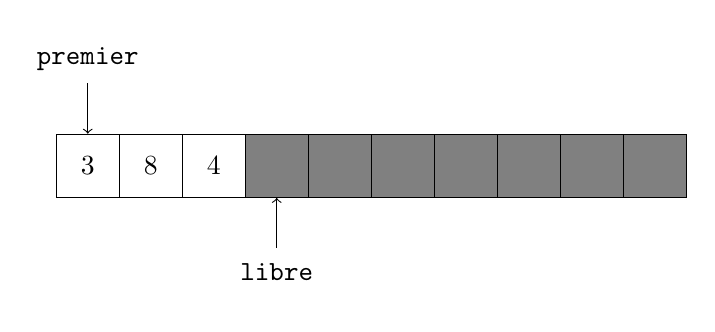
\begin{tikzpicture}[scale = 0.8,every node/.style={minimum size=0.8cm}]
\foreach \i/\v in {0/3,1/8,2/4}
  \node[draw] (t\i) at (\i, 0) {\v};
\foreach \i in {3,4,...,9}
    \node[draw,fill=gray] (t\i) at (\i cm, 0) {};
\draw [<-] (t0.north) -- +(0,0.8) node[above= -1mm]{\tt premier};
\draw [<-] (t3.south) -- +(0,-0.8) node[below= -1mm]{\tt libre};
\end{tikzpicture}
\end{center}
%--------------------------------------------------------------------------
\item On retire un élément (cela renvoie 3).
%--------------------------------------------------------------------------
\begin{center}
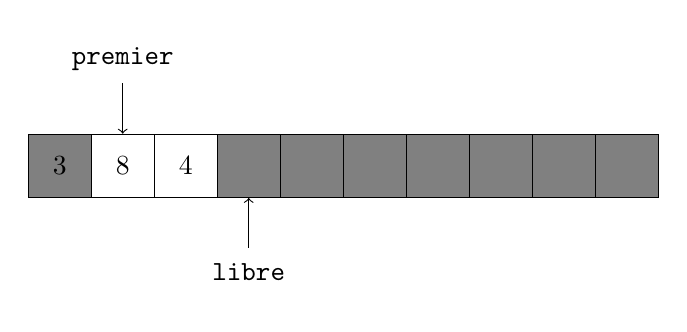
\begin{tikzpicture}[scale = 0.8,every node/.style={minimum size=0.8cm}]
\foreach \i/\v in {0/3}
  \node[draw,fill=gray] (t\i) at (\i, 0) {\v};
\foreach \i/\v in {1/8,2/4}
  \node[draw] (t\i) at (\i, 0) {\v};
\foreach \i in {3,4,...,9}
    \node[draw,fill=gray] (t\i) at (\i cm, 0) {};
\draw [<-] (t1.north) -- +(0,0.8) node[above= -1mm]{\tt premier};
\draw [<-] (t3.south) -- +(0,-0.8) node[below= -1mm]{\tt libre};
\end{tikzpicture}
\end{center}
%--------------------------------------------------------------------------
\item On ajoute 7.
%--------------------------------------------------------------------------
\begin{center}
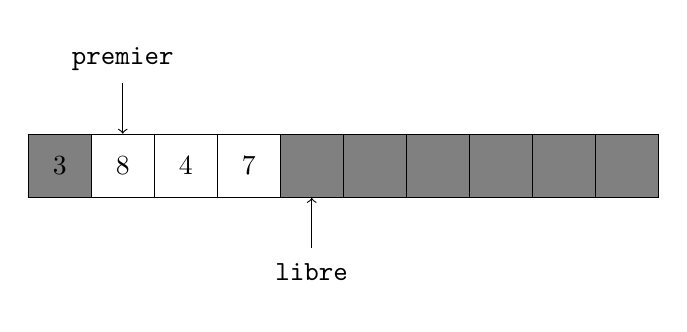
\begin{tikzpicture}[scale = 0.8,every node/.style={minimum size=0.8cm}]
\foreach \i/\v in {0/3}
  \node[draw,fill=gray] (t\i) at (\i, 0) {\v};
\foreach \i/\v in {1/8,2/4,3/7}
  \node[draw] (t\i) at (\i, 0) {\v};
\foreach \i in {4,5,...,9}
    \node[draw,fill=gray] (t\i) at (\i cm, 0) {};
\draw [<-] (t1.north) -- +(0,0.8) node[above= -1mm]{\tt premier};
\draw [<-] (t4.south) -- +(0,-0.8) node[below= -1mm]{\tt libre};
\end{tikzpicture}
\end{center}
%--------------------------------------------------------------------------
\item On retire un élément (cela renvoie 8).
%--------------------------------------------------------------------------
\begin{center}
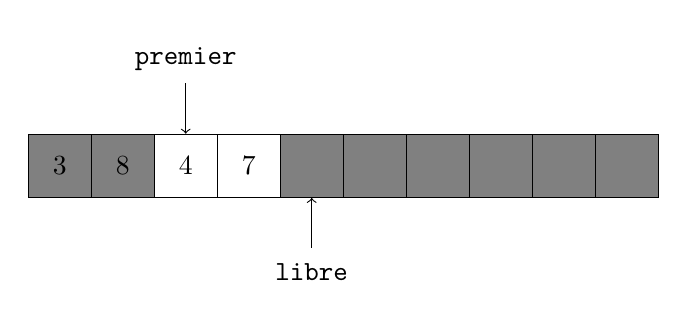
\begin{tikzpicture}[scale = 0.8,every node/.style={minimum size=0.8cm}]
\foreach \i/\v in {0/3,1/8}
  \node[draw,fill=gray] (t\i) at (\i, 0) {\v};
\foreach \i/\v in {2/4,3/7}
  \node[draw] (t\i) at (\i, 0) {\v};
\foreach \i in {4,5,...,9}
    \node[draw,fill=gray] (t\i) at (\i cm, 0) {};
\draw [<-] (t2.north) -- +(0,0.8) node[above= -1mm]{\tt premier};
\draw [<-] (t4.south) -- +(0,-0.8) node[below= -1mm]{\tt libre};
\end{tikzpicture}
\end{center}
%--------------------------------------------------------------------------
\end{itemize} 

On peut créer un dictionnaire avec des composantes sous la forme
%---------------------------------------------------------------------------
\begin{lstlisting}
dico = {"données" : [0]*nMax, "premier" : 0, "libre" : 0}
\end{lstlisting}
%---------------------------------------------------------------------------

Les composantes seront accessibles respectivement par \type{dico["données"]}, 

\type{dico["premier"]} ou \type{dico["libre"]}. 
%-------------------------------------------------------------------------------
%-------------------------------------------------------------------------------
\begin{Exercise}[title = {Implémentations d'une file à l'aide d'une liste}]\it

Donner des codes python pour les fonctions  \type{createQueue},  \type{emptyQueue},  \type{enque} et \type{deque} avec le modèle décrit ci-dessus.
\end{Exercise} 
%-------------------------------------------------------------------------------
\begin{Answer}
Pour comprendre le cas d'une liste vide on peut enlever tous les éléments et remarquer qu'alors \type{dico["premier"] = dico["libre"]}. On peut donc initialiser avec la valeur 0 pour \type{premier} et pour \type{libre}.
\begin{lstlisting}
def createQueue():
    nMax = 1000
    liste = [0]*nMax
    return {"données" : liste, "premier" : 0, "libre" : 0}
\end{lstlisting}

\begin{lstlisting}
def emptyQueue(file):
    return file["premier"] == file["libre"]
\end{lstlisting}

\begin{lstlisting}
def enque(x, file):
    nMax = len(file["données"])
    k = file["libre"]
    if k == nMax:
       print('La file est pleine')
    else:
        f["données"][k] = x
        f["libre"] = k + 1
\end{lstlisting}

\begin{lstlisting}
def deque(file):
    if emptyQueue(file):
        print('La file est vide')
    else:
        k = file["premier"]
        x = file["données"][k]
        f["premier"] = k + 1
        return x
\end{lstlisting}
\end{Answer}
%-------------------------------------------------------------------------------
\newpage
%--------------------------------------------------------------------------
\subsection{Implémentations des files par des tableaux "circulaires"}
%--------------------------------------------------------------------------
Dans l'implémentation ci-dessus on a le problème, déjà vu avec les piles, d'une taille maximale.

Cependant la situation est plus gênante ici : on peut avoir une file qui est vide est pleine à la fois, cela correspond au cas où toutes les positions ont été attribués et traités : on a alors \type{dico["premier"]} et \type{dico["libre"]} égaux à la taille du tableau. 

La solution pratique est de recommencer les numéros d'attente au début (on remet un nouveau distributeur de tickets).

\medskip

Dans l'exemple ci-dessus on suppose qu"on a ajouté encore les éléments 11, $-3$, 5, $-9$, 1, 17 et retiré deux fois un élément (cela renvoie 4 puis 7).
On arrive au tableau
%--------------------------------------------------------------------------
\begin{center}
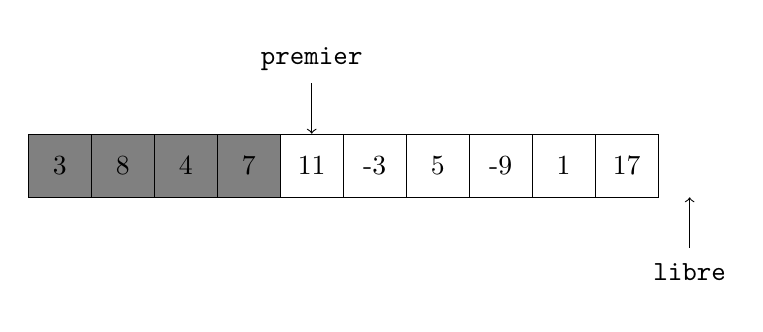
\begin{tikzpicture}[scale = 0.8,every node/.style={minimum size=0.8cm}]
\foreach \i/\v in {0/3, 1/8, 2/4, 3/7}
  \node[draw,fill=gray] (t\i) at (\i, 0) {\v};
\foreach \i/\v in {4/11, 5/-3, 6/5, 7/-9, 8/1, 9/17}
  \node[draw] (t\i) at (\i, 0) {\v};
%\foreach \i in {4,5,...,9}
%    \node[draw,fill=gray] (t\i) at (\i cm, 0) {};
\draw [<-] (t4.north) -- +(0,0.8) node[above= -1mm]{\tt premier};
\draw [<-] (10,-0.5) -- +(0,-0.8) node[below= -1mm]{\tt libre};
\end{tikzpicture}
\end{center}
%--------------------------------------------------------------------------

Pour pouvoir ajouter un élément on considère que le tableau est circulaire et que la place libre correspond à la position 0.
%--------------------------------------------------------------------------
\begin{center}
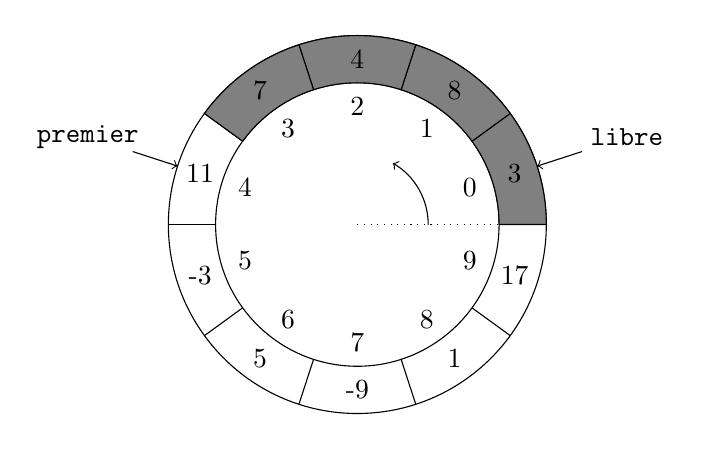
\begin{tikzpicture}[scale = 0.6]
\coordinate (O) at (0,0);
\draw (O) circle [radius=3cm];
\draw (O) circle [radius=4cm];
\foreach \k in {0,1,2,...,9}
  {\draw (\k*36:3)--(\k*36:4);
   \draw (\k*36+18:2.5) node {\k};
  };
\draw[dotted] (O) -- (0:4);
\draw[->] (0:1.5) arc (0:60:1.5);
\foreach \k/\n in {4/11, 5/-3, 6/5, 7/-9, 8/1, 9/17}
  \draw (\k*36+18:3.5) node {\n};
\foreach \k/\n in {0/3, 1/8, 2/4, 3/7}
  {\draw[fill=gray] (\k*36:3) -- (\k*36:4) arc (\k*36:\k*36+36:4) 
                              -- (\k*36+36:3) arc (\k*36+36:\k*36:3);
   \draw (\k*36+18:3.5) node {\n};};
\draw[->] (10*36+18:5) --(10*36+18:4);
\draw (10*36+18:6) node {\tt libre};
\draw[->] (4*36+18:5) --(4*36+18:4);
\draw (4*36+18:6) node {\tt premier};
\end{tikzpicture}
\end{center}%--------------------------------------------------------------------------
On peut alors ajouter des éléments, 14 et 21 par exemple et en retirer un (on obtient 11).
%--------------------------------------------------------------------------
\begin{center}
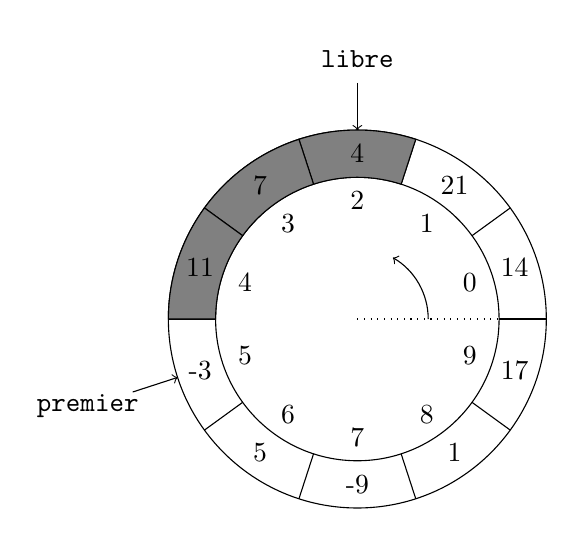
\begin{tikzpicture}[scale = 0.6]
\coordinate (O) at (0,0);
\draw (O) circle [radius=3cm];
\draw (O) circle [radius=4cm];
\foreach \k in {0,1,2,...,9}
  {\draw (\k*36:3)--(\k*36:4);
   \draw (\k*36+18:2.5) node {\k};
  };
\draw[dotted] (O) -- (0:4);
\draw[->] (0:1.5) arc (0:60:1.5);
\foreach \k/\n in {5/-3, 6/5, 7/-9, 8/1, 9/17, 0/14, 1/21}
  \draw (\k*36+18:3.5) node {\n};
\foreach \k/\n in {2/4, 3/7, 4/11}
  {\draw[fill=gray] (\k*36:3) -- (\k*36:4) arc (\k*36:\k*36+36:4) 
                              -- (\k*36+36:3) arc (\k*36+36:\k*36:3);
   \draw (\k*36+18:3.5) node {\n};};
\draw[->] (2*36+18:5) --(2*36+18:4);
\draw (2*36+18:5.5) node {\tt libre};
\draw[->] (5*36+18:5) --(5*36+18:4);
\draw (5*36+18:6) node {\tt premier};
\end{tikzpicture}
\end{center}
%--------------------------------------------------------------------------
Ce qui correspond au tableau
%--------------------------------------------------------------------------
\begin{center}
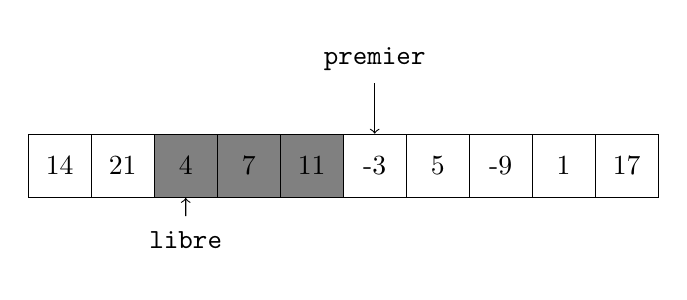
\begin{tikzpicture}[scale = 0.8,every node/.style={minimum size=0.8cm}]
\foreach \i/\v in {2/4, 3/7, 4/11}
  \node[draw,fill=gray] (t\i) at (\i, 0) {\v};
\foreach \i/\v in {5/-3, 6/5, 7/-9, 8/1, 9/17, 0/14, 1/21}
  \node[draw] (t\i) at (\i, 0) {\v};
\draw [<-] (t5.north) -- +(0,0.8) node[above= -1mm]{\tt premier};
\draw [<-] (t2) -- +(0,-0.8) node[below= -1mm]{\tt libre};
\end{tikzpicture}
\end{center}%-------------------------------------------------------------------------------
%-------------------------------------------------------------------------------
\begin{Exercise}[title = {Implémentations d'une file à d'une liste circulaire}]\it 

Donner des codes python pour les fonctions  \type{createQueue},  \type{emptyQueue},  \type{enque} et \type{deque} avec le modèle décrit ci-dessus.
\end{Exercise} 
%-------------------------------------------------------------------------------
\begin{Answer}
Il risque d'y avoir ambiguïté entre la notion de pile vide et pleine si la fin est une case avant le début. On "sacrifie" une case et on indique que la liste est vide si \type{dico["premier"] = dico["libre"]} et que la liste est pleine si \type{dico["premier"] = dico["libre"] +1}.

Les calculs doivent être fait avec le reste de la division par la taille du tableau.

\begin{lstlisting}
def createQueue():
    nMax = 1000
    liste = [0]*nMax
    return {"données" : liste, "premier" : 0, "libre" : 0}
\end{lstlisting}

\begin{lstlisting}
def emptyQueue(file):
    return file["premier"] == file["libre"]
\end{lstlisting}

\begin{lstlisting}
def enque(x, file):
    nMax = len(file["données"])
    k = file["libre"]
    p = file["premier"]
    if p== (k + 1)%nMax:
       print('La file est pleine')
    else:
        f["données"][k] = x
        f["libre"] = (k + 1)%nMax
\end{lstlisting}

\begin{lstlisting}
def deque(file):
    nMax = len(file["données"])
    if emptyQueue(file):
        print('La file est vide')
    else:
        p = file["premier"]
        x = file["données"][p]
        f["premier"] = (p + 1)%nMax
        return x
\end{lstlisting}
\end{Answer}%-------------------------------------------------------------------------------
%--------------------------------------------------------------------------
%--------------------------------------------------------------------------
\subsection{Implémentations des files par des objets python}
%--------------------------------------------------------------------------
On peut voir une file comme une chaîne de valeurs dont les deux extrémités sont accessibles.

%--------------------------------------------------------------------------
\begin{center}
\begin{tikzpicture}[scale = 0.8,grand/.style={minimum height=0.8cm, minimum width=1.6cm}]
\foreach \i/\v in {0/4, 1/7, 2/11, 3/-4}
  \node[grand,draw] (t\i) at (4*\i, 0) {\v};
\foreach \i in {1,2,3}
  {\pgfmathsetmacro\j{int(\i - 1)}
  \draw (t\i) -- (t\j);};
\draw [<-] (t0.north) -- +(0,0.8) node[above= -1mm]{\tt premier};
\draw [<-] (t3.north) -- +(0,0.8) node[above= -1mm]{\tt dernier};
\end{tikzpicture}
\end{center}%-------------------------------------------------------------------------------
En plus de la structure vue pour les piles il faut pouvoir enlever le premier élément donc chaque élément de la file doit accéder à l'élément suivant.

%--------------------------------------------------------------------------
\begin{center}
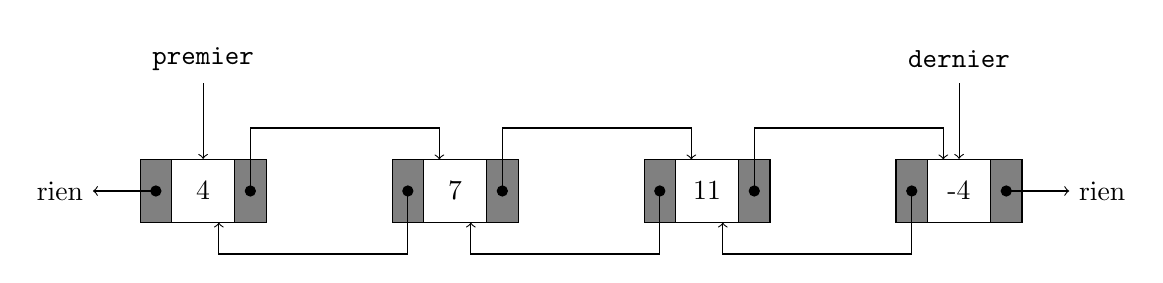
\begin{tikzpicture}[scale = 0.8,
                  grand/.style={minimum height=0.8cm, minimum width=1.6cm},
                  petit/.style={minimum size=0.8cm}]
\foreach \i/\v in {0/4, 1/7, 2/11, 3/-4}
  {\node[grand,draw,fill=gray] (t\i) at (4*\i, 0) {};
   \node[petit,draw,fill=white] (tt\i) at (4*\i, 0) {\v};};
\foreach \i in {0,1,2,3}
  {\draw[fill] (\i*4+0.75,0) circle (0.08);
   \draw[fill] (\i*4-0.75,0) circle (0.08);};
\foreach \i in {0,1,2}
   \draw[->] (\i*4+0.75,0) -- ++(0,1) -| ++(3,-0.5);
\foreach \i in {1,2,3}
   \draw[->] (\i*4-0.75,0) -- ++(0,-1) -| ++(-3,0.5);
\draw[->] (-0.75,0) -- ++(-1,0) node[left] {rien};
\draw[->] (4*3+0.75,0) -- ++(1,0) node[right] {rien};
\draw [<-] (t0.north) -- +(0,1.2) node[above= -1mm]{\tt premier};
\draw [<-] (t3.north) -- +(0,1.2) node[above= -1mm]{\tt dernier};
\end{tikzpicture}
\end{center}%-------------------------------------------------------------------------------
 On modifie donc les éléments et on définit la classe des files.
\begin{lstlisting}
class ElementFile:
    def __init__(elem,x):
        elem.valeur = x
        elem.suiv = None
        elem.prec = None
        
class File:
    def __init__(file):
        file.premier = None
        file.dernier = None
\end{lstlisting}

Comme on a deux position il faudra gérer spécifiquement les cas où on ajoute un élément à une file vide et où on retire son élément d'une file réduite à un élément.
%-------------------------------------------------------------------------------
%-------------------------------------------------------------------------------
\begin{Exercise}[title = {Implémentations d'une file à l'aide d'objets}]\it 

Donner des codes python pour les fonctions  \type{createQueue},  \type{emptyQueue},  \type{enque} et \type{deque} avec le modèle décrit ci-dessus.
\end{Exercise} 
%-------------------------------------------------------------------------------
\begin{Answer}
\begin{lstlisting}
def createQueue():
    return File()
\end{lstlisting}

\begin{lstlisting}
def emptyQueue(file):
    return file.premier is None
\end{lstlisting}

\begin{lstlisting}
def enque(x, file):
    e = ElementFile(x)
    if emptyQueue(file):
        file.premier = x
    else:
        penult = file.dernier
        e.prec = penult
        penult.suiv = e
    file.dernier = e
\end{lstlisting}
\newpage
\begin{lstlisting}
def deque(file):
    if emptyQueue(file):
        print("La file est vide")
    else:
        prem = file.premier
        if prem.suiv == None:
            file.dernier = None
        file.premier = prem.suiv
        return prem.valeur
\end{lstlisting}
\end{Answer}
%-------------------------------------------------------------------------------
\newpage
%-------------------------------------------------------------------------------
\subsection{File de priorité}
%---------------------------------------------------------------------------
%--------------------------------------------------------------------------
Une {\bf file de priorité} est une collection de données où les éléments sont comparables deux à deux. On souhaite enlever le plus grand (ou le plus petit) lorsque l'on retire un élément.
C'est la structure qui permet de gérer les traitements de données en tenant compte de priorités.

Par exemple les tâches qu'un processeur accomplit ont une priorité : le traitement d'un fichier à imprimer est moins important que l'affichage d'un film. On retrouve aussi la notion de file de priorité dans le traitement des urgences dans hôpital.

En informatique certains algorithmes, dits gloutons, doivent choisir à chaque étape un élément qui réalise un optimum, ils utiliseront souvent des files de priorités.
%--------------------------------------------------------------------------
\begin{center}
\begin{tikzpicture}
 \node[state] (s11) at (2,0) {$3$};
 \node[state] (s12) at (2,1) {$7$};
 \node[state] (s13) at (0.5,4) {$6$};
 \draw (1.5,3)-- ++(0,-3.5) -- ++(1,0) -- ++(0,3.5);
 \draw [->](s13.east) -| ++(1,-1.5);
%
 \node[state] (s21) at (4,0) {$3$};
 \node[state] (s22) at (4,1) {$7$};
 \node[state] (s23) at (4,2) {$6$};
 \draw (3.5,3)-- ++(0,-3.5) -- ++(1,0) -- ++(0,3.5);
%
 \node[state] (s31) at (6,0) {$3$};
 \node[state] (s32) at (6,1) {$6$};
 \node[state] (s33) at (7.5,4) {$7$};
 \draw (5.5,3)-- ++(0,-3.5) -- ++(1,0) -- ++(0,3.5);
 \draw [->](6,2.5) |- (s33.west);
\end{tikzpicture}
\end{center}
%--------------------------------------------------------------------------
Dans la pratique on utilisera des couples \type{(x ,k)} où $x$ est un élément et $k$ sa priorité.

{\bf Opérations :}
\begin{itemize}
\item \type{creerFP()} : retourne une file vide 
\item \type{ajouterFP(x, k, fileP)} : ajoute un élément $x$ de priorité $k$ dans la file $f$.
\item \type{enleverFP(fileP)} : supprime un élément de priorité maximale de la file et le renvoie.
\item \type{videFP(fileP)} : renvoie \type{True} si la file est vide, \type{False} sinon.
 \end{itemize}

On va utiliser des tableaux pour implémenter cette structure. On a alors un choix à faire : 

\begin{itemize}
\item on peut trier les éléments lors de l'adjonction, l'extraction est alors facilitée,
\item on peut adjoindre simplement les éléments, il faudra alors chercher le maximum lors de l'extraction.
\end{itemize} 
Chacune de ces deux options demande de parcourir la liste dans une des deux fonctions. Quand la file de priorité a $n$ éléments la complexité est donc de l'ordre de $n$. Il existe des structures de données plus sophistiquées qui permettent un accès plus rapide, de complexité ${\cal O}\bigl(\ln(n)\bigr)$.
%-------------------------------------------------------------------------------
%-------------------------------------------------------------------------------
\begin{Exercise}[title = {File de priorité avec des listes triées}]\it 

En s'inspirant de la fonction d'insertion vue lors du tri par insertion implémenter une structure de file de priorité qui utilise des listes triées.
\end{Exercise} 
%-------------------------------------------------------------------------------
\begin{Answer}
\begin{lstlisting}
def creerFP() :
    return []
\end{lstlisting}

\begin{lstlisting}
def videFP(fileP):
    return f == []
\end{lstlisting}

\begin{lstlisting}
def ajouterFP(x, fileP):
    fileP.append(x)
    i = len(f) -1
    while i > 0 and fileP[i][1] < fileP[i-1][1]:
        fileP[i] = fileP[i-1]
        i = i - 1
    fileP[i] = x
\end{lstlisting}

\begin{lstlisting}
def enleverFP(fileP):
    if videFP(fileP):
        return "La file est vide"
    else:
        return fileP.pop()
\end{lstlisting}
\end{Answer}%-------------------------------------------------------------------------------
%-------------------------------------------------------------------------------
\begin{Exercise}[title = {File de priorité avec des listes non triées}]\it

En utilisant une fonction de recherche du maximum implémenter une structure de file de priorité.\end{Exercise} 
%-------------------------------------------------------------------------------
\begin{Answer}
\begin{lstlisting}
def creerFP() :
    return []
\end{lstlisting}

\begin{lstlisting}
def videFP(fileP):
    return f == []
\end{lstlisting}

\begin{lstlisting}
def ajouterFP(x, fileP):
    fileP.append(x)
\end{lstlisting}

\begin{lstlisting}
def enleverFP(fileP):
    if videFP(fileP):
        return "La file est vide"
    else:
        n = len(fileP)
        max = fileP[0][1]
        iMax = 0
        for i in range(1,n):
            x, k = fileP[i]
            if k > max:
                max = k
                imax = i
        echange(fileP, iMax, n-1)
        return fileP.pop()

\end{lstlisting}
\end{Answer}
%-------------------------------------------------------------------------------
\newpage
%-------------------------------------------------------------------------------
\subsection{Ensembles}
%---------------------------------------------------------------------------
Un {\bf ensemble} est une collection de données où chaque élément ne peut apparaître qu'une seule fois. L'ordre d'entrée des éléments n'est pas pris en compte. Si on veut enlever un élément, il faut préciser sa valeur.
{\bf Opérations :}
\begin{itemize}
\item \type{ensembleVide()} : retourne un ensemble vide 
\item \type{videEns(e) } : renvoie vrai si l'ensemble est vide, faux sinon
\item \type{cardinal(e)} : renvoie le nombre d'éléments dans l'ensemble.
\item \type{appartient(x, e)} : renvoie \type{True} si $x\in e$ et \type{False} sinon.
\item \type{ajouterEns(x, e)} : ajoute un élément $x$ dans l'ensemble $e$ s'il n'était pas déjà un élément de $e$.
\item \type{enleverEns(x ,e)} : supprime un élément $x$ passé en entrée d'un ensemble $e$. Si $x$ n'appartenant pas à $e$, $e$ est inchangé.
\item \type{ensVersListe(e)} : transforme l'ensemble en liste afin de pouvoir parcourir les éléments.
\end{itemize}
%-------------------------------------------------------------------------------
%-------------------------------------------------------------------------------
\begin{Exercise}[title = {Ensemble avec des listes}]\it 

Implémenter une structure d'ensemble avec des listes.
\end{Exercise} 
%-------------------------------------------------------------------------------
\begin{Answer}
\begin{lstlisting}
def ensembleVide() :
    return []
\end{lstlisting}

\begin{lstlisting}
def videEns(e):
    return e == []
\end{lstlisting}

\begin{lstlisting}
def cardinal(e):
    return len(e)
\end{lstlisting}

\begin{lstlisting}
def appartient(x, e):
    for y in e:
        if x == y:
            return True
    return False
\end{lstlisting}

\begin{lstlisting}
def ajouterEns(x, e):
    if not appartient(x,e):
        e.append(x)
\end{lstlisting}

\begin{lstlisting}
def enleverEns(x, e):
    n = len(e)
    continue  = True
    i = 0
    while i < n and continue:
        if e[i] == x:
            echange(e, i, n-1)
            e.pop()
            continue  = False
\end{lstlisting}

\begin{lstlisting}
from copy import deepcopy
def ensVersListe(e):
    return deepcopy(e)
\end{lstlisting}
\end{Answer}
%-------------------------------------------------------------------------------
%-------------------------------------------------------------------------------

\medskip

Il arrivera parfois que les ensembles considérés soient des sous-ensemble d'un ensemble fixé.
On considérera que l'ensemble de base est $\{0,1,2,\ldots,n-1\}$ et on pourra représenter un sous-ensemble par un tableau de booléens : 

\type{e[i]} vaut \type{True} si et seulement si $i$ appartient à $e$.
%-------------------------------------------------------------------------------
%-------------------------------------------------------------------------------
\begin{Exercise}[title = {Ensemble avec des tableaux de booléens}]\it

Implémenter une structure d'ensemble comme sous-ensembles de $\{0,1\ldots,n-1\}$.

La fonction \type{ensembleVide} admettra la taille de l'ensemble initial comme paramètre optionnel.
\end{Exercise} 
%-------------------------------------------------------------------------------
\begin{Answer}
\begin{lstlisting}
def ensembleVide(n=1000) :
    return [False]*n
\end{lstlisting}

\begin{lstlisting}
def cardinal(e):
    n = len(e)
    card = 0
    for i in range(n):
        if e[i]:
            card = card + 1
    return card
\end{lstlisting}

\begin{lstlisting}
def estEnsVide(e):
    return cardinal(e) == 0
\end{lstlisting}

\begin{lstlisting}
def ajouterEns(x, e):
    e[x] = True
\end{lstlisting}

\begin{lstlisting}
def enleverEns(x, e):
    e[x] = False
\end{lstlisting}

\begin{lstlisting}
def ensVersListe(e):
    n = len(e)
    return [i for i in range(n) if e[i]]
\end{lstlisting}
\end{Answer}
%-------------------------------------------------------------------------------
%-------------------------------------------------------------------------------
%-------------------------------------------------------------------------------
%-------------------------------------------------------------------------------

\newpage
%-------------------------------------------------------------------------------
%------------------------------------------------------------
%------------------------------------------------------------
%------------------------------------------------------------
%------------------------------------------------------------
%------------------------------------------------------------
